\documentclass[sigplan,preprint,10pt]{acmart}\settopmatter{printfolios=true,printccs=false,printacmref=false}
\settopmatter{printacmref=false} 
\renewcommand\footnotetextcopyrightpermission[1]{}
\pagestyle{plain} 

\usepackage{lineno,hyperref,xcolor}
\usepackage{flushend}
\usepackage{stmaryrd}
\usepackage{amssymb}
\usepackage{xypic}
\usepackage{semantic}
\usepackage{booktabs} 
\usepackage{subcaption}
\usepackage{enumitem}
\usepackage[shortlabels]{enumerate}
\setlist{leftmargin=6mm}

\newcounter{thc}
\newcounter{dfc}

\theoremstyle{plain}
\newtheorem{lem}[thc]{Lemma}
\newtheorem{theorem}[thc]{Theorem}

\theoremstyle{definition}
\newtheorem{definition}[dfc]{Definition}

%\acmConference[PL'17]{ACM SIGPLAN Conference on Programming Languages}{January 01--03, 2017}{New York, NY, USA}
%\acmYear{2017}
%\acmISBN{} % \acmISBN{978-x-xxxx-xxxx-x/YY/MM}
%\acmDOI{} % \acmDOI{10.1145/nnnnnnn.nnnnnnn}
\startPage{1}
\setcopyright{none}
\bibliographystyle{ACM-Reference-Format}

\title{Wrattler: \textnormal{A platform for AI-assisted data science}}

\author{Authors}
%\affiliation{
%  \institution{The Alan Turing Institute}
%  \country{London, United Kingdom}
%}
%\email{tomas@tomasp.net}


\definecolor{cmtclr}{rgb}{0.0,0.6,0.0}
\definecolor{kvdclr}{rgb}{0.0,0.0,0.6}
\definecolor{numclr}{rgb}{0.0,0.4,0.0}
\definecolor{strclr}{rgb}{0.4,0.4,0.0}
\definecolor{rstrclr}{rgb}{0.5,0.1,0.0}
\definecolor{prepclr}{rgb}{0.6,0.0,0.2}
\newcommand{\vect}[1]{\langl #1 \rangl}
\newcommand{\langl}{\begin{picture}(4.5,7)
\put(1.1,2.5){\rotatebox{60}{\line(1,0){5.5}}}
\put(1.1,2.5){\rotatebox{300}{\line(1,0){5.5}}}
\end{picture}}
\newcommand{\rangl}{\begin{picture}(4.5,7)
\put(.9,2.5){\rotatebox{120}{\line(1,0){5.5}}}
\put(.9,2.5){\rotatebox{240}{\line(1,0){5.5}}}
\end{picture}}
\newcommand{\ball}[1]{\FPeval{\result}{clip(201+#1)}\textnormal{\ding{\result}}}
\newcommand{\lsep}{~\,|\,~}
\newcommand{\num}[1]{\textcolor{numclr}{#1}}
\newcommand{\str}[1]{\textnormal{\textcolor{strclr}{\sffamily "#1"}}}
\newcommand{\rstr}[1]{\textnormal{\textcolor{rstrclr}{\sffamily "#1"}}}
\newcommand{\ident}[1]{\textnormal{\sffamily #1}}
\newcommand{\qident}[1]{\textnormal{\sffamily \guillemotleft #1\guillemotright}}
\newcommand{\dom}{\ident{dom}}
\newcommand{\kvd}[1]{\textnormal{\textcolor{kvdclr}{\sffamily #1}}}

\newcommand{\bndclr}[1]{\textcolor{kvdclr}{#1}}
\newcommand{\bkndclr}[1]{\textcolor{prepclr}{#1}}
\newcommand{\blblclr}[1]{\textcolor{numclr}{#1}}
\newcommand{\bnd}[1]{\textnormal{\textcolor{kvdclr}{\sffamily #1}}}
\newcommand{\bknd}[1]{\textnormal{\textcolor{prepclr}{\sffamily #1}}}
\newcommand{\blbl}[1]{\textnormal{\textcolor{numclr}{\sffamily #1}}}


\begin{document}
\maketitle

\section{Introduction}
Data science is an iterative, exploratory process that requires a collaboration between a 
computer system and a human. A computer can run a machine learning algorithm to provide advice 
based on statistical analysis of the data and discover hidden structures or corner cases, but only
a human can decide what those mean.
A data science environment of the future thus needs to support an interaction model that 
keeps the human in the loop, allows an efficient interaction between the human and the computer
and can be extended with new AI asistants that provide advice about data.

In this report, we present Wrattler, a notebook system that is interactive, reproducible, 
polyglot and smart.

\paragraph{Interactive.}
Wrattler enables an efficient interaction by bringing computation closer to the human.
Notebooks run in the browser, cache partial results of computations and provide previews
of script results on-the-fly during development.

\paragraph{Reproducible.} 
Wrattler separates the task of running scripts from the task of managing state.
A data store tracks the provenance and semantics of data, supports versioning and keeps 
the history, making the data analyses fully reproducible.

\paragraph{Polyglot.}
The use of data store makes it possible to combine multiple programming languages in 
a single notebook. Data scientists can mix interactive languages for quick data exploration
that run in the web browser and provide live previews with robust systems such as R and Python.

\paragraph{Smart.}
Last, but not least, Wrattler serves as a platform for AI assistants that use novel
machine learning algorithms to provide suggestions about data. Such AI assistants connect to the
data store to infer types and meaning of data, provide help with data cleaning and joining, but also help data scientists
make sense of data by finding typical and atypical data points and automatically visualizing data.

\section{Wrattler and notebooks}

Notebook systems such as Jupyter became a popular programming environment for data science, because 
they support gradual data exploration and provide a convenient way of interleaving code with 
comments and visualizations. However, notebooks suffer from a number of issues that hanper 
reproducibility, make it difficult to combine multiple languages and limit the possible interaction
model.

Notebooks can be used in a way that breaks reproducibility. The state is maintained by a \emph{kernel} 
and running a code in a cell overwrites the current state. There is no record of how the current 
state was obtained and no way to rollback to a previous state. The fact that the state is 
maintained by the kernel means that it is hard to combine multiple programming languages and
other components such as AI assistants. Finally, notebooks provide a very limited interaction 
model. To see the effect of a code change, an entire cell and all subsequent cells need to be
manually reevalutated.

\begin{figure}
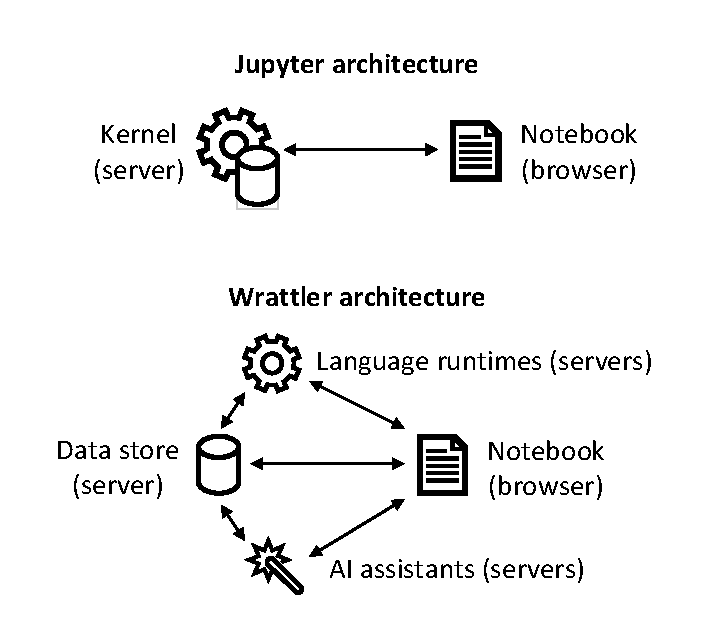
\includegraphics[scale=0.6]{diagram.pdf}
\caption{In notebook systems such as Jupyter, state and execution is managed by a kernel. In
  Wrattler, those functions are separated and enriched with AI assistants.}
\label{fig:arch}
\end{figure}

The architecture of Wrattler allows us to address these issues, as well as to provide a platform
for building novel AI assistants and interactive programming. The architecture is illustrated
in Figure~\ref{fig:arch}. The components of Wrattler are:
%
\begin{itemize}
\item[--] \textbf{Data store}. Imported external data, results of running scripts and of 
  applying AI assistants are stored in the data store. It stores versioned data frames with 
  other semantic information about data such as types, semantics, data format or provenance.
\vspace{0.25em}
\item[--] \textbf{Language runtimes}. Scripts are evaluated by one or more language runtimes.
  The runtimes read input data from and write results back to the data store.
\vspace{0.25em}
\item[--] \textbf{AI assistants}. When invoked from the notebook, AI assistants read data
  from data store and provide hints to the data analyst. They help to write data cleaning
  scripts or annotate data in the data store with additional metadata such as inferred types.
\vspace{0.25em}
\item[--] \textbf{Notebook}. The notebook is displayed in a web browser, which orchestrates 
  all other components. The browser builds a dependency graph between cells or individual 
  expressions in the cells. It calls language runtimes to evaluate code that has changed
  and reads data from the data store to display results.  
\end{itemize}

\section{Wrattler components}

b

\subsection{Notebook user interface}

\subsection{Dependency graph}

\subsection{Data store}

\subsection{Language runtimes}

\subsection{AI assistants}

\newpage
~
\newpage

platform for AI-assisted data science that  
Wrattler - an experimental notebook system that addresses the above issues. Wrattler is
 based on a simple idea of moving the state from a single language-specific stateful kernel
  to a datastore that can communicate with multiple workers that evaluate code or provide insights about data.
  
  I will discuss the far reaching consequences that the Wrattler architecture has. First, we can 
  provide live previews by recomputing only parts of notebooks. Second, our notebooks track 
  history and are fully reproducible. Third, it becomes possible to mix multiple languages and 
  also integrate AI assistants that communicate directly with the datastore to provide 
  suggestions about data extraction, cleaning and integration.


% context
% problem
% how we solve it
% what follows

Data science properties
What follows from this
Notebook issues
Wrattler architecture
What this enables






























\end{document}
